\section{Geometria del piano}

\subsection{Angoli}

\begin{questions}

	\begin{qblock}
		\question
		\exonly{
			Convertire in forma sessagesimale:
		}

		\begin{parts}
			\part
			\exonly{\ang{5,645}}  \solonly{\ang{5;38;42}}

			\part
			\exonly{\ang{15,37}}  \solonly{\ang{15;22;12}}

			\part
			\exonly{\ang{8,8}}  \solonly{\ang{8;48;}}
		\end{parts}
	\end{qblock}

	\begin{qblock}
		\question
		\exonly{

			Convertire in gradi (forma decimale):
		}

		\begin{parts}
			\part
			\exonly{\ang{4;47;8} } \solonly{\ang{4.786}}

			\part
			\exonly{\ang{;895;}}  \solonly{\ang{14.92}}

			\part
			\exonly{\ang{12;38;24}}  \solonly{\ang{12.64}}
		\end{parts}
	\end{qblock}

	\begin{qblock}
		\question
		\exonly{

			Convertire in gradi (forma decimale):
		}

		\begin{parts}
			\part
			\exonly{$\dfrac{\pi}{2}$} \solonly{\ang{90}}

			\part
			\exonly{$\dfrac{2}{3}\pi$}  \solonly{\ang{120}}

			\part
			\exonly{$\dfrac{5}{3}\pi$}  \solonly{\ang{300}}
		\end{parts}
	\end{qblock}

	\begin{qblock}
		\question
		\exonly{

			Convertire in radianti (valore esatto):
		}

		\begin{parts}
			\part
			\exonly{\ang{30} } \solonly{$\dfrac{\pi}{6}$}

			\part
			\exonly{\ang{135}}  \solonly{$\dfrac{3}{4}\pi$}

		\end{parts}
	\end{qblock}

	\begin{qblock}
		\question
		\exonly{
			Calcolare l'angolo $\epsilon$ tra l'altezza $BH$ e la bisettrice $BI$ del vertice $B$.
		}

		\begin{parts}
			\part
			\exonly{
				Nel caso particolare dove  $\angle ABC = 60^\circ$ e $\angle BCA= 40{}^\circ$.}
			\solonly{$\epsilon=\ang{20}$}
			\part
			\exonly{In generale in funzione di  $\angle ABC = \alpha$ e $\angle BCA= \beta$ }
			\solonly{$\epsilon=90 -\frac{\alpha}{2}-\beta$}
		\end{parts}


		\exonly{
			\begin{tikzpicture}[line cap=round,line join=round,>=triangle 45,x=1.0cm,y=1.0cm,rotate=-30]
				\draw (-1.0,3.0) node[left] {B}-- (3.0,3.0);
				\draw (3.0,3.0) node[below right] {H}-- (3.0,0.0) ;
				\draw (3.0,0.0) node[below] {A}-- (-1.0,3.0);
				\draw (3.0,4.0)-- (-1.0,3.0);
				\draw (3.0,4.0)-- (3.0,3.0);
				\draw (3.0,6.0) node[right] {C}-- (3.0,4.0) node[below right] {I};
				\draw (3.0,6.0)-- (-1.0,3.0) ;
				\draw (2.8,3)--(2.8,3.2)--(3,3.2);
				\draw (0,3) arc (0:14.04:1) node[right,midway,yshift=-0.1cm] {$\epsilon$} ;
			\end{tikzpicture}
		}
	\end{qblock}

	\begin{qblock}
		\question
		\exonly{
			Calcolare gli angoli $\gamma$ e $\delta$  in funzione di $\alpha$ e $\beta$:
			%Calculer les angles $\gamma$ et $\delta$ en fonction de $\alpha$ et $\beta$ :
		}

		\begin{parts}
			\part \exonly{
				se $ \alpha = 20^\circ$  e  $ \beta = 40^\circ$.}
			\solonly{$\gamma=\ang{30}$ \quad  $\delta=\ang{30}$
			}
			\part \exonly{per $\alpha$ e $\beta$ qualunque.}
			\solonly{$\gamma=\delta=90-\alpha -\beta$
			}
		\end{parts}

		\includegraphics*[width=0.5\linewidth]{ch1-ex3}
	\end{qblock}

\end{questions}

\subsection{Triangoli simili}

\begin{questions}

	\begin{qblock}
		\question
		\exonly{
			Calcolare le misure mancanti $a$, $b$, $c$, $d$, $x$ e $y$ (in $\SI{}{\centi\meter}$) nei casi seguenti. Le rette $f$ e $g$ sono parallele.
		}

		\exonly{\includegraphics*[width=0.5\linewidth]{ch2-ex3-1}}

		\begin{parts}
			\part
			\exonly{$a=\num{4.5}$ \quad $b=?$ \quad $c=3$  \quad  $d=2$ \\ $x=3$ \quad $y=?$}
			\solonly{$b=3$ \quad $y=5$}

			\part
			\exonly{$a=\num{6}$ \quad $b=?$ \quad $c=?$  \quad  $d=\num{1.6}$ \\ $x=5$ \quad $y=7$}
			\solonly{$b=\num{2.4}$ \quad $c=4$}

			\part
			\exonly{$a=?$ \quad $b=\num{4.2}$ \quad $c=\num{6.8}$  \quad  $d=\num{5.1}$ \\ $x=?$ \quad $y=\num{6.4}$}
			\solonly{$a=\num{5.6}$ \quad $x=\num{3.66}$}

			\part

			\exonly{ $a=?$ \quad $b=\num{5.2}$ \quad $c=\num{2.8}$  \quad  $d=?$ \\ $x=\num{4.2}$ \quad $y=\num{8.1}$}
			\solonly{$a=\num{5.6}$\quad $d=\num{2.6}$}

			\part
			\exonly{$a=2$ \quad $b=\frac{7}{3}$ \quad $c=\frac{3}{2}$  \quad  $d=?$ \\ $x=\frac{6}{5}$ \quad $y=?$}
			\solonly{$d=\frac{7}{4}=\num{1.75}$ \quad$y=\frac{13}{5}=\num{2.6}$}

		\end{parts}
	\end{qblock}

	\begin{qblock}
		\question
		\exonly{
			A causa del lago non é possibile misurare la distanza $AC$.
			Per poter calcolare questa distanza determiniamo i punti $B_1$ e $C_1$ tali per cui $B_1C_1$ sia parallela a $BC$.

			Possiamo quindi misurare:

			$AB_{1}=\SI{15}{\meter}$ ~ $AC_{1}= \SI{9}{\meter}$ ~ $BB_{1}= \SI{133}{\meter}$.

			Calcolare la distanza  $AC$.

		}
		\solonly{$AC=\SI{88.8}{\meter}$}

		%TODO : convert in TikZ
		\exonly{\includegraphics*[width=0.5\linewidth]{ch2-ex2}}
	\end{qblock}

	\begin{qblock}
		\question
		\exonly{
			Per determinare l'altezza di un palazzo un uomo si posiziona in modo da vedere la cima di un palo allineata alla cima del palazzo (altezza degli occhi  $\approx \SI{1.65}{\meter}$).

			La distanza tra il palo (di altezza $\SI{3}{\meter}$) e il palazzo é di $\SI{33}{\meter}$ e quella tra il palo e la persone é di $\SI{7}{\meter}$


			Calcolare l'altezza $h$ del palazzo.
		}

		\exonly{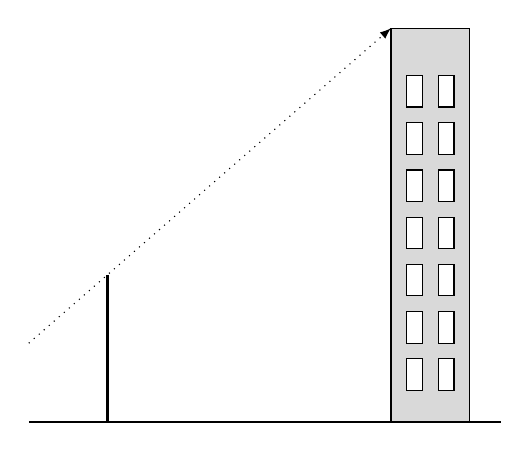
\begin{tikzpicture}
				\human[0.5]{A}{0,0.5}
				\draw[thick] (0,0) --(6,0);
				\filldraw[fill=gray!30] (4.6,0) rectangle (5.6,5);
				\draw[very thick] (1,0) -- (1,1.87);
				%\draw[dotted,latex-latex] (0,1) -- node[above, midway] {\num{23.5}} (4.6,1);
				\foreach \x in {0.2,0.8,1.4,2,2.6,3.2,3.8}
					{
						\filldraw[fill=white] (4.8, \x + 0.2) rectangle +(0.2,0.4) (5.2,0.2 + \x) rectangle +(0.2,0.4) ;
					}
				\draw[dotted,-latex] (0,1) -- (4.6,5);


			\end{tikzpicture}}
		%\exonly{\includegraphics*[width=\linewidth]{ch2-ex7}}
		\solonly{$h=\SI{9.36}{\meter}$}
	\end{qblock}
\end{questions}

\subsection{Triangolo rettangolo}

\begin{questions}

	\begin{qblock}
		\question
		\exonly{ %Borgeaud 2.7.1. a)

			Calcolare i lati e gli angoli mancanti del triangolo qui sotto:
		}

		\ifprintanswers   \else

			%\hspace*{-3cm}
			\begin{tikzpicture}[scale=1.3]
				\tkzInit[xmin=-1,xmax=5,ymin=-5,ymax=0.5]
				\tkzClip
				\tkzDefPoint(0,0){A}
				\tkzDefShiftPoint[A](-90:4.1){B}
				\tkzDefShiftPoint[B](0:1.9){C}
				\tkzDrawPolygon(A,B,C)
				\tkzLabelPoints[above](A)
				\tkzLabelPoints[below](B,C)
				\tkzLabelSegment[above right](C,A){$b$}
				\tkzLabelSegment[below](C,B){\SI{19}{\meter}}
				\tkzLabelSegment[left](A,B){\SI{41}{\meter}}
				\tkzDefLine[orthogonal=through B](C,A) \tkzGetPoint{h1}
				\tkzInterLL(C,A)(B,h1) \tkzGetPoint{H}
				\tkzDrawSegment(B,H)
				\tkzLabelSegment[above left](H,B){$h$}
				\tkzMarkRightAngle(B,H,A)
				\tkzMarkRightAngle(C,B,A)
				%\tkzLabelAngle[pos=0.7](A,C,B){$\gamma$}
				%\tkzMarkAngle[arc=l,size=.5 cm](A,C,B)
				%\tkzLabelAngle[pos=0.7](C,B,A){$\beta$}
				%\tkzMarkAngle[arc=l,size=.5 cm](C,B,A)
				%
				%\tkzLabelAngle[pos=0.7](C,A,B){$\alpha$}
				%\tkzMarkAngle[arc=l,size=.5 cm](B,A,C)
			\end{tikzpicture}
		\fi

		\solonly{$b=\SI{45.19}{\meter}$ \quad $\angle BCA=\ang{65.14}$  \\ $\angle CAB= \ang{24.86}$  \quad $h=\SI{17.24}{\meter}$
		}
	\end{qblock}

	\begin{qblock}
		\question
		\exonly{%Borgeaud 2.7.1. b)
			Calcolare i lati e gli angoli mancanti del triangolo qui sotto:}

		\ifprintanswers   \else
			\begin{tikzpicture}[scale=1.5]
				\tkzDefPoint(0,0){C}
				\tkzDefShiftPoint[C](-90:4.1){A}
				\tkzDefShiftPoint[C](0:1.9){B}
				\tkzDrawPolygon(A,B,C)
				\tkzLabelPoints[above](C,B)
				\tkzLabelPoints[below](A)
				\tkzLabelSegment[left](C,A){$b$}
				\tkzLabelSegment[above](C,B){$a$}
				\tkzLabelSegment[right](A,B){\SI{105}{\meter}}
				\tkzLabelAngle[pos=1](B,A,C){$\ang{38}$}
				\tkzMarkAngle[arc=l,size=.5 cm](B,A,C)
				\tkzMarkRightAngle(B,C,A)
			\end{tikzpicture}
		\fi

		\solonly{$b=\SI{82.74}{\meter}$  $\angle CBA=\ang{52}$  \\ $a=\SI{64.64}{\meter}$
		}
	\end{qblock}

	\begin{qblock}
		\question
		\exonly{ %Borgeaud 2.7.1. c)
			Calcolare i lati e gli angoli mancanti del triangolo qui sotto:
		}

		\ifprintanswers   \else

			\begin{tikzpicture}[scale=1.5]
				\tkzDefPoint(0,0){A}
				\tkzDefShiftPoint[A](-90:3){B}
				\tkzDefShiftPoint[B](0:4){C}
				\tkzDrawPolygon(A,B,C)
				\tkzLabelPoints[below](C,B)
				\tkzLabelPoints[above](A)
				\tkzLabelSegment[above right](C,A){$b$}
				\tkzLabelSegment[below](C,B){\SI{30}{\meter}}
				\tkzLabelSegment[left](A,B){\SI{25}{\meter}}
				\tkzMarkRightAngle(C,B,A)
			\end{tikzpicture}
		\fi

		\solonly{$b=\SI{39.05}{\meter}$  $\angle BCA=\ang{39.81}$  \\ $\angle BAC=\ang{50.19}$
		}
	\end{qblock}

	\begin{qblock}
		\question
		\exonly{%Borgeaud 2.7.1. d)
			Calcolare i lati e gli angoli mancanti del triangolo qui sotto:
		}

		\ifprintanswers   \else
			\begin{tikzpicture}[scale=0.8]
				\tkzDefPoint(0,0){A}
				\tkzDefShiftPoint[A](-90:3){B}
				\tkzDefShiftPoint[B](0:8){C}
				\tkzDrawPolygon(A,B,C)
				\tkzLabelPoints[below](C,B)
				\tkzLabelPoints[above](A)
				\tkzLabelSegment[above right](C,A){\SI{50}{\meter}}
				\tkzLabelSegment[below](C,B){$a$}
				\tkzLabelSegment[left](A,B){$c$}
				\tkzMarkRightAngle(C,B,A)
				\tkzLabelAngle[pos=1.1](B,A,C){\footnotesize $1,2^{rad}$}
				\tkzMarkAngle[arc=l,size=.5 cm](B,A,C)
			\end{tikzpicture}
		\fi

		\solonly{$a=\SI{46.6}{\meter}$  $\angle BCA=\ang{21.25}$  \\ $c=\SI{18.12}{\meter}$
		}
	\end{qblock}

	\begin{qblock}
		\question
		\exonly{%Borgeaud 2.7.4


			Qual'é l'altezza di una torre che proietta al suolo un ombra di \SI{96}{\metre} quando il sole forma un angolo \ang{52.5}  di con l'orizzonte?

		}
		\solonly{$\SI{125.11}{\meter}$}
	\end{qblock}

	\begin{qblock}
		\question
		\exonly{%Borgeaud 2.7.5

			Determinare l'angolo formato dai raggi di sole e l'orizzonte se  l'ombra di un palo vale  $\num{1.5}$ volte la sua altezza?

		}

		\solonly{\ang{33.69}}
	\end{qblock}

\end{questions}

\subsection{Angolo al centro}

\begin{questions}

	\begin{qblock}
		\question
		\exonly{Calcolare $\alpha$, $\beta$, $\gamma$ e $\delta$.}

		\exonly{
			%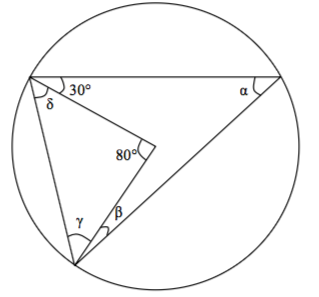
\includegraphics[width=0.5\linewidth]{aac-1}
			\pgfmathsetmacro\radius{4}
			\begin{tikzpicture}
				\coordinate[label=below right:$O$] (O) at (0,0);
				\draw (O) circle (\radius);
				\filldraw (O) circle (1pt);
				\coordinate (A) at (20:\radius);
				\coordinate (B) at (150:\radius);
				\coordinate (C) at (250:\radius);

				\draw (A) -- (B) -- (C)-- cycle;
				\draw (B) -- (O)-- (C);

				\draw pic["$\alpha$",draw, angle eccentricity=1.3,angle radius=1cm] {angle=B--A--C};
				\draw pic["$\beta$",draw, angle eccentricity=1.3,angle radius=1cm] {angle=A--C--O};
				\draw pic["$\gamma$",draw, angle eccentricity=1.3,angle radius=0.6cm] {angle=O--C--B};
				\draw pic["$\delta$",draw, angle eccentricity=1.3,angle radius=0.6cm] {angle=C--B--O};
				\draw pic["$30^{\circ}$",draw, angle eccentricity=1.4,angle radius=1cm] {angle=O--B--A};
				\draw pic["$80^{\circ}$",draw, angle eccentricity=1.4,angle radius=1cm] {angle=B--O--C};
			\end{tikzpicture}

		}

		\solonly{$\alpha=40^{\circ}$, $\gamma=\delta=50^{\circ}$, $\beta=10^{\circ}$}
	\end{qblock}

	\begin{qblock}
		\question
		\exonly{Calcolare $\alpha$, $\beta$, $\gamma$ e $\delta$.}

		\exonly{
			\begin{tikzpicture}
				\pgfmathsetmacro\radius{4}
				\coordinate[label=below right:$O$] (O) at (0,0);
				\draw[name path=circle] (O) circle (\radius);
				\filldraw (O) circle (1pt);
				\coordinate (A) at (120:\radius);
				\coordinate (B) at (250:\radius);
				\coordinate (C) at (\radius+4,2);


				\draw[name path=l1] (A) --  (C);
				\draw[name path=l2] (B) -- (C);

				\path [name intersections={of=l1 and circle,by={A1}}];
				\path [name intersections={of=l2 and circle,by={B1}}];

				\draw[name path=s1] (A) -- (B1);
				\draw[name path=s2] (B) -- (A1);
				\path [name intersections={of=s1 and s2,by={S}}];


				\draw pic [draw,angle radius=3mm] {right angle = B1--S--B};

				\draw pic["$\alpha$",draw, angle eccentricity=1.3,angle radius=0.6cm] {angle=A--A1--S};
				\draw pic["$\beta$",draw, angle eccentricity=1.3,angle radius=0.6cm] {angle=S--B1--B};
				\draw pic["$\gamma$",draw, angle eccentricity=1.3,angle radius=0.8cm] {angle=B1--B--S};
				\draw pic["$\delta$",draw, angle eccentricity=1.3,angle radius=0.6cm] {angle=A--C--B};
				\draw pic["$20^{\circ}$",draw, angle eccentricity=1.4,angle radius=1cm] {angle=S--A--A1};
			\end{tikzpicture}


			%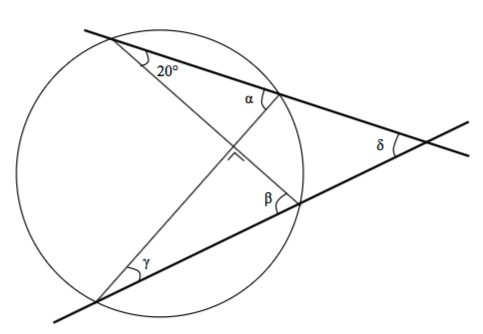
\includegraphics[width=0.6\linewidth]{aac-2}
		}

		\solonly{$\gamma=20^{\circ}$, $\alpha=\beta=70^{\circ}$, $\delta=50^{\circ}$}
	\end{qblock}

\end{questions}

\subsection{Triangoli qualunque}

\begin{questions}

	\begin{qblock}
		\question
		\exonly{
			Calcolare l'area dei triangoli qui sotto nelle situazioni date:
			%	Calculer l'aire du triangle ci-dessous pour le situations suivantes:
		}

		\ifprintanswers   \else
			%\begin{adjustbox}{width=\linewidth}
			\begin{tikzpicture}%[every node/.style={opacity=1, black, above left}] 
				\path (0,0) coordinate (A)  node[left] {$A$};
				\path (5,0) coordinate (B) node[right] {$B$};
				\path (3,2) coordinate (C) node[above] {$C$};
				\path (A) -- (B) node[midway,below] {$c$};
				\path (B) -- (C) node[midway,above] {$a$};
				\path (C) -- (A) node[midway,above] {$b$};
				%\path ($(A)!0.5!(B)$) node [below] {$c$} ;
				%\node at ($(A)!0.5!(B)$) [below] {$c$}  ;
				%\node at ($(A)!0.5!(C)$) [above ] {$b$}  ;
				%\node at ($(C)!0.5!(B)$) [above] {$a$}  ;
				\draw (A)--(B)--(C) --cycle;
				\path
				pic[pic text=$\alpha$,draw,angle eccentricity=1.5] {angle=B--A--C}
				pic[pic text=$\beta$,draw,angle eccentricity=1.5] {angle=C--B--A}
				pic[pic text=$\gamma$,draw,angle eccentricity=1.5] {angle=A--C--B}
				;

			\end{tikzpicture}
		\fi

		\begin{parts}
			\part \exonly{$\alpha=\ang{40}$, $b=\SI{38}{\meter}$, $c=\SI{25}{\meter}$}
			\solonly{\SI{305.32}{\square\meter}}

			\part
			\exonly{$\alpha =\ang{31}$, $\gamma=\ang{40}$, $a=\SI{53}{\meter}$}
			\solonly{\SI{1657.47}{\square\meter}}

		\end{parts}
	\end{qblock}

	\begin{qblock}
		\question
		\exonly{
			Calcolare $\alpha$, $\beta$ e $\gamma$.
		}


		\ifprintanswers   \else

			\begin{tikzpicture}[scale=0.7]
				\coordinate[label=below :$B$]  (B) at (0,0);
				\coordinate[label= right:$C$]  (C) at (35:5);
				\coordinate[label=above:$A$]  (A) at (100:6);
				\draw (A) -- node[midway, left] {$\SI{7}{\meter}$} (B) --node[midway, below right] {$\SI{5}{\meter}$} (C) --node[midway, above right] {$\SI{6}{\meter}$} cycle;
				\path
				pic[pic text=$\alpha$,draw,angle eccentricity=1.5] {angle=B--A--C}
				pic[pic text=$\beta$,draw,angle eccentricity=1.5] {angle=C--B--A}
				pic[pic text=$\gamma$,draw,angle eccentricity=1.5] {angle=A--C--B};
			\end{tikzpicture}
		\fi

		\solonly{$\alpha \approx \num{44.42}^{\circ}$, $\beta \approx \num{57.12}^{\circ}$, $\gamma \approx \num{78.46}^{\circ}$}
	\end{qblock}

	\begin{qblock}
		\question
		\exonly{
			Calcolare $c$, $\beta$ e $\gamma$.}

		\ifprintanswers   \else

			\begin{tikzpicture}[scale=0.7]
				\coordinate[label=below :$B$]  (B) at (0,0);
				\coordinate[label= right:$C$]  (C) at (0:5);
				\coordinate[label=above:$A$]  (A) at (76:6);
				\draw (A) -- node[midway, left] {$c$} (B) --node[midway, below ] {$\SI{5}{\meter}$} (C) --node[midway, above right] {$\SI{7}{\meter}$} cycle;
				\path
				pic[pic text=$35\degree$,draw,angle eccentricity=1.5] {angle=B--A--C}
				pic[pic text=$\beta$,draw,angle eccentricity=1.5] {angle=C--B--A}
				pic[pic text=$\gamma$,draw,angle eccentricity=1.5] {angle=A--C--B};
			\end{tikzpicture}
		\fi

		\solonly{$\beta_1 \approx \num{53.42}^{\circ}$, $\gamma_1 \approx \num{91.58}^{\circ}$, $c_1\approx \SI{8.71}{\meter}$}

		\solonly{$\beta_2 \approx \num{126.58}^{\circ}$, $\gamma_2 \approx \num{18.42}^{\circ}$, $c_2\approx \SI{2.75}{\meter}$}
	\end{qblock}

	\begin{qblock}
		\question
		\exonly{
			Calcolare $c$, $\alpha$, $\beta$ e $\gamma$ se l'area del triangolo é di $\SI{12}{\square\meter}$.
		}

		\exonly{

			\begin{tikzpicture}[scale=0.8]
				\coordinate[label=below :$B$]  (B) at (0,0);
				\coordinate[label= right:$C$]  (C) at (0:3);
				\coordinate[label=above:$A$]  (A) at (64:5);
				\draw (A) -- node[midway, left] {$c$} (B) --node[midway, below ] {$\SI{6}{\meter}$} (C) --node[midway, above right] {$\SI{5}{\meter}$} cycle;
				\path
				pic[pic text=$\alpha$,draw,angle eccentricity=1.5] {angle=B--A--C}
				pic[pic text=$\beta$,draw,angle eccentricity=1.5] {angle=C--B--A}
				pic[pic text=$\gamma$,draw,angle eccentricity=1.5] {angle=A--C--B};
			\end{tikzpicture}
		}

		\solonly{$\alpha_1 \approx \ang{73.74}$, $\beta_1 \approx \ang{53.13}$ \\$\gamma_1 \approx \ang{53.13}$, $c_1\approx \SI{5}{\meter}$}

		\solonly{$\alpha_2 \approx \ang{29.16}$, $\beta_2 \approx \ang{23.97}$ \\ $\gamma_2 \approx \ang{126.87}$, $c_2\approx \SI{9.85}{\meter}$}
	\end{qblock}

	\begin{qblock}
		\question
		\exonly{
			Per stimare l'altezza di una montagna per triangolazione un osservatore misura l'angolo di elevazione $\alpha=\ang{25}$ (angolo tra l'orizzontale e la cima della montagna). In seguito, spostandosi sullo sullo stesso piano, si avvicina  percorre $d=\SI{1000}{\meter}$ in direzione della montagna  e misura di nuovo l'angolo di elevazione che ora é di $\beta=\ang{38}$.

			Stimare l'altezza $h$ della montagna rispetto al piano sul quali si trova l'osservatore.

		}

		\solonly{$h=\SI{1156.65}{\meter}$}
	\end{qblock}

	\begin{qblock}
		\question
		\exonly{

			La torre di Pisa ha un'inclinazione di \ang{10;15;} rispetto alla verticale.
			Quando é inclinata verso il sole, i cui raggi formano un angolo di \ang{33} con l'orizzonte, l'ombra della torre misura \SI{74.9}{\meter}.

			Qual'era l'altezza originale della torre?


		}

		\solonly{$h=\SI{56}{\meter}$
		}
	\end{qblock}

	\subsection{Poligoni e cerchi}

	\begin{questions}

		\begin{qblock}
			\question
			\ifprintanswers \else
				Calcolare la lunghezza $L_1$.% e $L_2$.

				\begin{minipage}{0.4\textwidth}
					\begin{tikzpicture}
						\coordinate (O) at (0,0);
						\coordinate (B) at (120:2.5);
						\coordinate (A) at (0:2.5);
						\draw (A) -- node[midway, below] {$r=\SI{2.5}{\meter}$} (O) -- (B);
						\path
						pic[pic text=$120\degree$,draw,angle eccentricity=1.5] {angle=A--O--B};
						\draw[dashed] (O) circle (2.5);
						\draw[very thick] (A) arc (0:120:2.5) node[midway, above] {$L_1$} ;
					\end{tikzpicture}


				\end{minipage}


			\fi


			\solonly{$L_1=\SI{5.24}{\meter}$ }%\qquad $L_2=\SI{26.18}{\meter}$}
		\end{qblock}

		\begin{qblock}
			\question
			\exonly{
				L'estremità di un pendolo di \SI{60}{\centi\meter} descrive, oscillando, un arco di \SI{17}{\centi\meter}.

				Calcolare l'angolo percorso dal file del pendolo durante un oscillazione.
			}

			\solonly{ \ang{16.23}}
		\end{qblock}

		\begin{qblock}
			\question
			\exonly{
				Calcolare la lunghezza della strada (le parti curve sono archi di cerchio).

				%	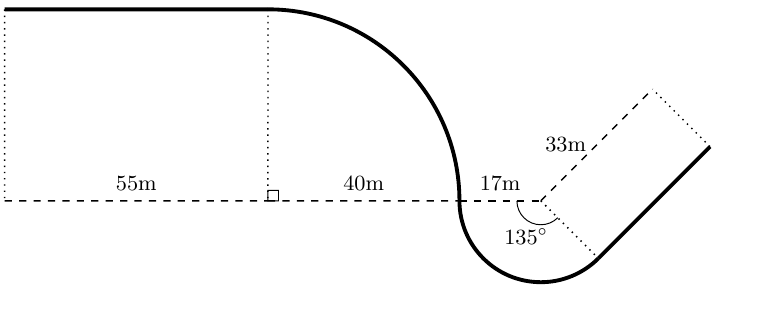
\includegraphics[scale=1]{es1-5-3}

				\begin{tikzpicture}[scale=0.7]
					\tkzDefPoint(0,0){O}
					\tkzDefPoint(-5.7,0){O1}
					\tkzDefShiftPoint[O](-1.7,0){P3}
					\tkzDefShiftPoint[P3](-4,4){P2}
					\tkzDefShiftPoint[P2](0,-4){P2a}
					\tkzDefShiftPoint[P2](-5.5,0){P1}
					\tkzDefShiftPoint[P1](0,-4){P1a}
					\tkzDefShiftPoint[O](-45:1.7){P4}
					\tkzDefShiftPoint[P4](45:3.3){P5}
					\tkzDefShiftPoint[P5](135:1.7){P5a}
					\tkzDrawSegments[ultra thick,color=black](P1,P2 P4,P5)
					\tkzDrawArc[ultra thick,color=black](O,P3)(P4)
					\tkzDrawArc[ultra thick,color=black](O1,P3)(P2)
					\tkzDrawSegments[dashed,color=black](P1a,P2a   P2a,P3 P3,O  O,P5a)
					\tkzDrawSegments[dotted,color=black](P1,P1a P2,P2a  O,P4  P5,P5a)
					\tkzLabelSegment(P1a,P2a){\footnotesize $55$m}
					\tkzLabelSegment(P3,P2a){\footnotesize  $40$m}
					\tkzLabelSegment(P3,O){\footnotesize  $17$m}
					\tkzLabelSegment[left](O,P5a){\footnotesize $33$m}
					\tkzMarkAngle[arc=l,size=0.5 cm,](P3,O,P4)
					\tkzLabelAngle[pos=0.8,circle](P3,O,P4){\footnotesize  $135^\circ$}
					\tkzMarkRightAngle(P2,P2a,P3)
				\end{tikzpicture}
				%TODO diegno in tikz

			}

			\solonly{$\SI{190.89}{\meter}$}
		\end{qblock}

		\begin{qblock}
			\question
			\exonly{
				I rettangoli  $R_1$, $R_2$, $R_3$ e $R_4$ hanno la stessa area.

				Calcolare l'area e il perimetro della figura.

				%TODO : convert in TikZ
				\begin{tikzpicture}
					\pgfmathsetmacro\l{8}
					\pgfmathsetmacro\h{6}

					\pgfmathsetmacro\p{2}

					\coordinate(O) at (0,0);
					\draw (O) rectangle (\l,\h);
					\draw (\p,0) rectangle (\l,\h);
					\draw (\p,0) rectangle (\l,\h-\p);
					\draw[] (\p,0) rectangle (\p+0.5*\l-0.5*\p,\h-\p);

					\dimline[extension start length=1cm,extension end length=1cm] {(\p,\h+0.5)}{(\l,\h+0.5)}{$12$ cm};
					\dimline[extension start length=-1cm,extension end length=
						-1cm] {(\l+0.5,0)}{(\l+0.5,\h-\p)}{$10$ cm};
					\coordinate[label=$R_1$] (R1) at (1,\h/2);
					\coordinate[label=$R_2$] (R2) at (5,4.55);
					\coordinate[label=$R_3$] (R2) at (3.5,2);
					\coordinate[label=$R_4$] (R2) at (6.5,2);
				\end{tikzpicture}

				%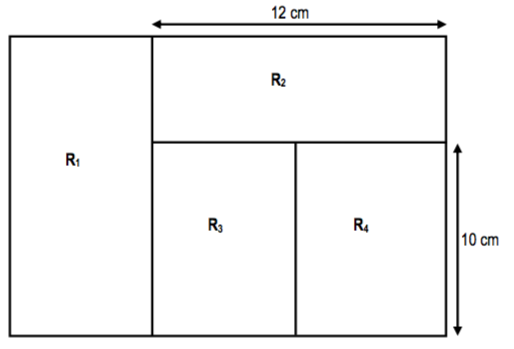
\includegraphics[width=0.5\linewidth]{surf-1}
			}

			\solonly{
				$A=\SI{240}{\square\centi\meter}$ \\
				$P=\SI{62}{\centi\metre}$
			}
		\end{qblock}

		\begin{qblock}
			\question
			\exonly{
				Calcolare l'area della superficie in grigio.
				Il lato del quadrato misura $\SI{10}{\centi\meter}$.
				$A$ e $B$ sono i centri degli archi di cerchio.

				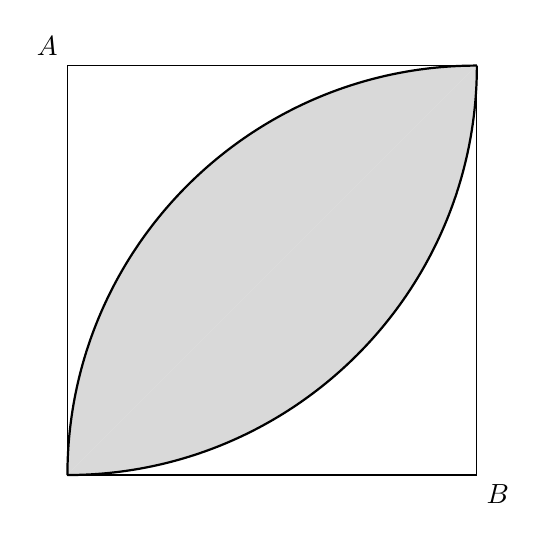
\begin{tikzpicture}[scale=1.3]
					\filldraw[gray!30] (4,0) arc (90:180:4) ;
					\filldraw[gray!30] (4,0) arc (0:-90:4);
					\draw (0,0) node[above left] {$A$} rectangle (4,-4) node[below right] {$B$};
					\draw[thick] (4,0) arc (90:180:4);
					\draw[thick] (4,0) arc (0:-90:4);
				\end{tikzpicture}
				%\includegraphics[width=0.6\linewidth]{surf-3}
			}


			\solonly{
				$A\approx\SI{57.08}{\square\centi\meter}$
			}
		\end{qblock}

		\begin{qblock}
			\question
			\exonly{
				Calcolare l'area della superficie in grigio.
				Il lato del quadrato misura $\SI{7}{\centi\meter}$.
				$A$ e $B$ sono i centri degli archi di cerchio.
			}

			\exonly{

				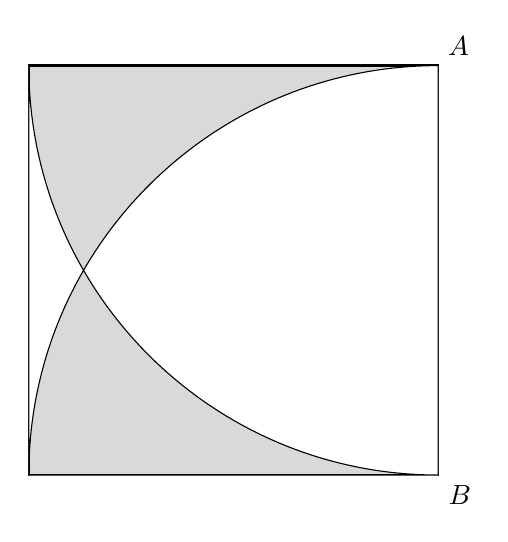
\begin{tikzpicture}[scale=1.3]
					\path (4,0) node[above right] {$A$} ;
					\filldraw[thick,draw=black,fill=gray!30] (0,0) rectangle (4,-4) node[below right] {$B$};

					\clip (0,0) rectangle (4,-4);
					\begin{scope}
						\filldraw[draw=black,fill=white,even odd rule] (0,0) rectangle (4,-4) (4,-4) circle (4) (4,0) circle (4) ;
					\end{scope}

				\end{tikzpicture}

				%\includegraphics[width=0.6\linewidth]{surf-5}
			}

			\solonly{
				$A\approx\SI{16.76}{\square\centi\meter}$
			}
		\end{qblock}

		\begin{qblock}
			\question
			\exonly{
				L'arco di cerchio (di centro $O$) qui sotto ha un angolo al centro di \ang{230}.
				La lunghezza della corda $AB$ é di $\SI{7}{\meter}$.

				Calcolare il raggio $R$ dell'arco di cerchio e l'altezza $H$.}

			\exonly{
				\begin{tikzpicture}[scale=0.8]
					\draw (0,0) node[above] {$O$} -- node[above, midway] {$R$} (15:4);
					\draw (-45:4) node[below] {$B$} arc (-45:225:4) node[below] {$A$};
					\draw (-45:4) --  + (0:2) -- +(180:8);
					\draw[dashed] (-45:4) ++(0:1.5) |- (0,4);
					\coordinate (A) at ({$(-45:4)+(0:1.5)$} |- {$(0,4)$});
					\draw[latex-latex, thick] (-45:4) ++(0:1.5) -- node[right,midway]{$H$}(A);

				\end{tikzpicture}


				%\includegraphics[width=\linewidth]{surf-6}
			}

			\solonly{
				$R\approx\SI{3.86}{\meter}$ , $H\approx\SI{5.49}{\meter}$
			}
		\end{qblock}

	\end{questions}

\end{questions}